\partsintesi{Síntesi de la Part II}{Anàlisi de funcions}

\begin{mylist}
	\exer[2] Calcula el domini de les següents funcions
	\begin{tasks}(2)
		\task $f(x)=\dfrac{1}{x^2+5x}$
		\task $f(x)=\sqrt{5-2x}$
	\end{tasks}
	\answers{a) $\mathbb{R}-\{0, -5\}$, b) $(-\infty, 5/2]$}
	
	\exer[2] Representa gràficament les següents funcions:
	\begin{tasks}(2)
		\task $y=|x^2 + 2x -3|$
		\task $y=\log_2(x-1)$
	\end{tasks}
	\answers{ a) 
		\includegraphics*[width=0.22\textwidth]{img-07-bloc2/bloc2-2a.png}
		\par
		b)	
		\includegraphics*[width=0.22\textwidth]{img-07-bloc2/bloc2-2b.png}}
	
	\exer[2] Siguin les funcions $f(x)=e^x$, $g(x)=\sin x$, $h(x)=\sqrt{x}$. Calcula les següents composicions: $g(h(x))$, $f(g(x))$, $h(f(x))$. Troba la funció inversa de $h(f(x))$.
	\answers{$g(h(x))=\sin \sqrt{x}$, $f(g(x))=e^{\sin x}$, $h(f(x))=\sqrt{e^x}$. $h(f(x))^{-1}=\ln x^2$.}
	
	\exer[2] Calcula els següents límits:
	\begin{tasks}(3)
		\task $\limx{1}\dfrac{x-1}{\sqrt{x+3}-2}$
		\task $\limx{-5}\dfrac{x^2+5}{x^2+7x+10}$
		\task $\limx{+\infty}\dfrac{2x-5x^3}{1+x^2}$
	\end{tasks}
	\answers{a) $4$, b) $\limx{-5^-} f(x)=+\infty$ i $\limx{-5^+} f(x)=-\infty$ , c) $-\infty$}
	
	\exer[2] Donada la funció a trossos $f(x)=\left\{ 
	\begin{array}{ll}
	3x-b & x<2 \\
	3    & x=2 \\
	-2x+9& x>2
	\end{array}
	\right.$
	\begin{tasks}
	\task Determina $b$ perquè existeixi el límit de la funció a $x=2$.
	\task Després, determina si la funció és contínua o no indicant, si escau, el tipus de  discontinuïtat.
	\end{tasks}
	\answers{a) $b=1$, b) $f$ és discontínua a $x=2$ per punt desplaçat.}
	
	\exer[2] Calcula, a partir de la definició, la derivada de la funció $f(x)=3x^2 -10x$ en el punt d'abscissa $x=3$. 
	\answers{$f'(3)=\limx[h]{0} \frac{f(3+h)-f(3)}{h}= \limx[h]{0} \frac{3(3+h)^2-10(3+h)-(-3)}{h} =8$.}
	
	\exer[2] Un cultiu de bacteris ve donat per l'expressió $y=100 \cdot e^{0.05\cdot t}$ on $y$ són el nombre de cèl·lules i $t$ el temps donat en minuts. 
	\begin{tasks}
		\task Calcula el nombre de bacteris inicial ($t=0$) i passat mitja hora.
		\task El temps que tardarien ha arribar a 5000 bacteris.
		\task Fes una gràfica de la funció.
	\end{tasks} 
	\answers{a) $y(0)=100$ bacteris, \par $y(30)=100\cdot e^{0.05\cdot 30}\approx 448$;  
		
		b) $5000 = 100\cdot e^{0.05\cdot t}$ $\rightarrow$ $0.05\cdot t = \ln(5000/100)$ $\rightarrow$  $t = \ln(50)/0.05 \approx 78,2 $
	
		c) Gràfica
	
	\includegraphics*[width=0.4\textwidth]{img-07-bloc2/bloc2-6.png}
}
	
	\exer[2] Escriu l'equació de la recta tangent a la corba $y=\dfrac{x-3}{x+2}$ en el punt d'abscissa \linebreak $x=1$.
	\answers{$y=-\frac{2}{3}+\frac{5}{9}(x-1)$ o $y=\frac{5x}{9}-\frac{11}{9}$.}
	
	\exer[2] Calcula la funció derivada de les següents funcions:
	\begin{tasks}(2)
		\task $y=\sqrt{\cos (5x^4+2x^3)}$
		\task $y=\frac{\ln x}{x^2}$
		\task $y=\arcsin (3x^5 - 6 x^2)$
		\task $y=x\cdot e^{-x^2}$
		\task $y=\left(\frac{2x+5}{3x-1}\right)^5$
		\task $y=\sqrt{x+\sqrt{x}}$
	\end{tasks}
	 \answers{\begin{tasks}
	 	\task $y'=-\frac{1}{2\sqrt{\cos(5x^4+2x^3)}}\cdot \sin(5x^4+2x^3) \cdot (20x^3+6x^2)$
	 	\task $y'=\frac{1-2\ln x}{x^3}$
	 	\task $y'=\frac{1}{\sqrt{1-(3x^5-6x^2)^2}}\cdot (15x^4-12x)$
	 	\task $y'=(1-2x^2)\cdot e^{-x^2}$
	 	\task $y'=-85\left( \frac{2x+5}{3x-1} \right)^4 \cdot \frac{1}{(3x-1)^2}$
	 	\task $y'=\frac{1}{2\sqrt{x+\sqrt{x}}}\cdot (1+\frac{1}{2\sqrt{x}})$
 \end{tasks}}
	
	\exer[2] Determina els intervals de creixement i decreixement, màxims i mínims de les funcions:
	\begin{tasks}(2)
		\task $y=x^3-12x$
		\task $y=\dfrac{x^2-4}{x}$
	\end{tasks}
\answers{a) Creixent: $(-\infty, -2)\cup (2,+\infty)$;  Decreixent $(-2,2)$; Màxims: $(x=-2,\, y=16)$; Mínims: $(x=2, y=-16)$.
	b)Sempre és creixent. No té extrems.}	

	\exer[2] Es considera la funció $y=x^4-x^3-6x^2$. Es demana:
\begin{tasks}
	\task Trobau els punts de tall amb els eixos
	\task Calculau els extrems relatius
	\task Feu una gràfica de la funció
\end{tasks}
\answers{Punts de tall amb l'eix OX:  $x=-2$, $x=0$, $x=3$, i amb l'eix OY $(0,0)$. Té un màxim a (0,0) i té dos mínims a $x=2.15$, $y=-16.3$ i a $x=-1.4$, $y=-5.2$
	La gràfica de la funció és:
	
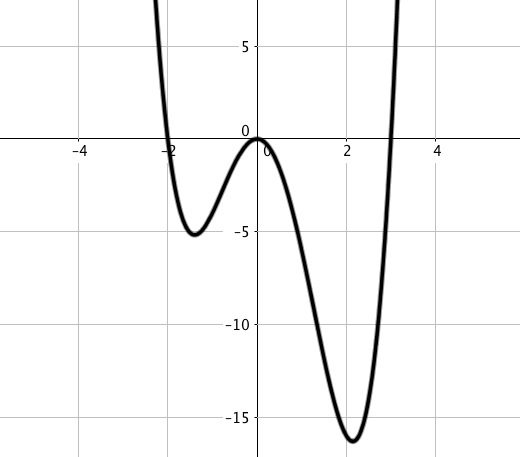
\includegraphics[width=0.3\textwidth]{img-07-bloc2/sol-bloc2-polinomi1.png}
}
	
	\exer[2] Donada la funció $y=\dfrac{x^2}{x^2-4x+3}$, calcula:
	\begin{tasks}
		\task Les asímptotes i la posició relativa de la corba respecte d'elles
		\task Els màxims i mínims relatius
		\task Representa la gràfica
	\end{tasks}
\answers{\begin{tasks}
		\task $y=1$ asímptota horitzontal; $x=1$ i $x=3$ asímptotes verticals. La posició relativa és: $\limx{+\infty} f(x)=1$ per damunt; 
		$\limx{-\infty} f(x)=1$ per davall. $\limx{1^-} f(x)=+\infty$, $\limx{1^+} f(x)=-\infty$, $\limx{3^-} f(x)=-\infty$, $\limx{3^+} f(x)=+\infty$.
		%
		\task La funció té un mínim relatiu a $x=0$, $y=0$ i un màxim relatiu a $x=3/2$, $y=-3$
		\task Gràfica: 	
	
		\includegraphics*[width=0.35\textwidth]{img-07-bloc2/bloc2-10.png}
		%
\end{tasks}}

	
	\exer[2] Quina d'aquestes funcions té una asímptota obliqua?
	\begin{tasks}(3)
		\task $y=\dfrac{x^2-4}{x^2}$
		\task $y=\dfrac{4+2x^3}{x}$
		\task $y=\dfrac{2x^2-1}{x-1}$
	\end{tasks}
	Calcula i representa totes les seves asímptotes.
	\answers{L'única funció que presenta asímptota obliqua és c). L'asímptota obliqua és $y=2x+2$ i també té una asímptota vertical a $x=1$. La gràfica és la següent:  
		
			\includegraphics*[width=0.4\textwidth]{img-07-bloc2/bloc2-11.png}
	}
	
	\exer[2] Trobau què ha de valer $k$ perquè la funció $y=2x-1$ sigui una asímptota obliqua de la funció $f(x)=\frac{2x^2-1}{x+k}$. En tal cas, determinau, si escau, els extrems relatius.
	\answers{ $k=1/2$. La primera derivada $y'=(2x^2+2x+1)/(x+1/2)^2$ mai és zero. Sempre creix i per tant no té extrems.}
	
	\exer[2] Calcula $a$ i $b$ perquè la funció  $y=x^3+ax^2+b$  tingui un punt d'inflexió en el punt \linebreak $P(2, 1)$.
	\answers{$a=-6$ i $b=17$.}

	
\end{mylist}


\newpage
%	\vspace*{-0.5cm}
%\subsection*{Resum del bloc de funcions}
	\vspace*{-0.25cm}
\begin{center}
		\vspace{-0.4cm}
	\setlength\LTleft{0pt}
	\setlength\LTright{0pt}
	\ftimes{10.5}{11}
	\fontsize{10.5}{11}
	\begin{longtable}[h]{|p{1.02\textwidth}|}
		\hline %inserts double horizontal lines
		\rowcolor{lightgray} \textbf{\textsc{Definició de funció}} \\   [0.5ex]   \hline
		$f(x)$: Domini $f \subset \mathbb{R} \rightarrow$ Recorregut $f\subset \mathbb{R}$, és una funció si per a cada valor de $x$ del domini s'assigna un únic valor de $y$ del recorregut. $y=f(x)$ ``$y$ (ordenada) és la imatge de $x$ (abscissa) per la funció $f$.\\
		\hline
	\end{longtable}
\end{center}
\vspace{-0.25cm}
\begin{center}
	\vspace{-1cm}
	\setlength\LTleft{0pt}
	\setlength\LTright{0pt}
	\ftimes{10.5}{11}
	\fontsize{10.5}{11}
	\begin{longtable}[h]{|p{0.323\textwidth}|p{0.323\textwidth}|p{0.323\textwidth}|}
		\hline %inserts double horizontal lines
	\rowcolor{lightgray} 	\multicolumn{3}{|l|}{\textbf{\textsc{Algunes funcions elementals}}} \\   [0.5ex]   \hline		
	Funció exponencial $y=a^x$, $e^x$ \par  \includegraphics*[width=0.25\textwidth]{img-07-bloc2/bloc2-pic1.png} & 
Funció trigonomètrica  $y=\sin x$ \par \includegraphics*[width=0.25\textwidth]{img-07-bloc2/bloc2-pic2.png} & 
Funció $y=\tg x$ \par \includegraphics*[width=0.25\textwidth]{img-07-bloc2/bloc2-pic3.png} 
\\ [0.5ex] \hline

Funció logarítmica   $y=\log_b x$ \par \includegraphics*[width=0.25\textwidth]{img-07-bloc2/bloc2-pic4.png}& 
$y=\cos x$ \par   \includegraphics*[width=0.25\textwidth]{img-07-bloc2/bloc2-pic5.png}  & Funció arctangent $y=\arctg x$\par  \includegraphics*[width=0.25\textwidth]{img-07-bloc2/bloc2-pic6.png}  \\ [0.5ex] \hline
	\end{longtable}
\end{center}
	\vspace{-1.5cm}
\begin{center}
	\setlength\LTleft{0pt}
	\setlength\LTright{0pt}
	\ftimes{10.5}{11}
	\fontsize{10.5}{11}
	\begin{longtable}[h]{|p{0.5\textwidth}|p{0.5\textwidth}|}
		\hline %inserts double horizontal lines
		\rowcolor{lightgray} \multicolumn{2}{|l|}{\textbf{\textsc{Càlcul de límits}} }\\   [0.5ex]   \hline
		 
		 \textsc{Límits Laterals}: El límit existeix si els dos límits laterals coincideixen.
		 
		 \begin{center}
		 	 \includegraphics*[width=0.25\textwidth]{img-07-bloc2/bloc2-pic7.png} 
		 \end{center}
		
		  &
		 \textsc{Límits a l'infinit}
		 
		 \begin{center}
			  \includegraphics*[width=0.4\textwidth]{img-07-bloc2/bloc2-pic8.png} 
		 \end{center}
		
		 \\ [0.5ex] \hline
		 
		 \multicolumn{2}{|p{\textwidth}|}{
			 Límits immediats: $\limx{4} \sqrt{x} = \sqrt{4}=2$;  $\limx{\pi/4} \tg x = tg \frac{\pi}{4}=1$; etc. \par
			 \textsc{\bf Indeterminacions}:\par
		 	  \begin{itemize}
		 	  	\exer[2] $\frac{0}{0}$: Factoritzar (o racionalitzar) i simplificar \par
		 	  		 $\limx{0} \frac{x^3-3x^2}{x^2} = \limx{0} \frac{x^2\cdot(x-3)}{x^2} = \limx{0} (x-3)=-3$;
		 	  		 $\limx{4} \frac{\sqrt{x}-2}{x-4} = \limx{4} \frac{(\sqrt{x}-2)(\sqrt{x}+2)}{(x-4)(\sqrt{x}+2)}= \cdots = 1/4$ \vspace{0.4cm}
		 	  	\exer[2] $\frac{\infty}{\infty}$: Dividir tots els termes per la major potència de $x$ del denominador \par
		 	  	  $\limx{+\infty} \frac{2x^2+1}{3x^2+x+1} = \limx{+\infty} \frac{2+1/x^2}{3+1/x+1/x^2}=\frac{2}{3}$;
		 	  	  \vspace{0.4cm}
		 	  	\exer[2] $0 \cdot \infty$: Es redueix al cas $\infty/\infty$ \par
		 	  	$\limx{+\infty} \frac{1}{x^2} \cdot (x^3-2x+1) = \limx{+\infty} \frac{x^3-2x+1}{x^2}=+\infty$;
		 	  	  \vspace{0.4cm}
		 	  	  \exer[2] $\infty-\infty$: Reduir a denominador comú i simplificar (racionalitzar si hi arrels) \par
		 	  	  $\limx{+\infty}\left( \frac{x^2}{x-2} - \frac{2x^3-3x+1}{2(x-2)}\right) = \limx{+\infty} \frac{2x^2-(2x^2-3x+1)}{2(x-2))}=\limx{+\infty} \frac{3x-1}{2x-4}=3/2$;
		 	  \end{itemize} 
	 	} \\ [0.5ex] \hline
 	
		 
	\end{longtable}
\end{center}
	\vspace{-0.5cm}
\begin{center}
 
	\setlength\LTleft{0pt}
	\setlength\LTright{0pt}
	\ftimes{10.5}{11}
	\fontsize{10.5}{11}
	\begin{longtable}[h]{|p{0.5\textwidth}|p{0.5\textwidth}|}
		\hline %inserts double horizontal lines
		\rowcolor{lightgray} \textbf{\textsc{Funció Contínua}} & \textbf{\textsc{Tipus de discontinuïtats}}
		\\ [0.5ex] \hline
		
		$f(x)$ és contínua en $x=a$ si
		
		\begin{enumerate}
			\exer[2] $\limx{a^-} f(x) =\limx{a^+} f(x) = \limx{a} f(x)$
			\exer[2] Existeix $f(a)$
			\exer[2] $\limx{a} f(x)=f(a)$
		\end{enumerate}
			
			&
			
			\begin{enumerate}
			\exer[2] Asimptòtica. $\limx{a} f(x)=\pm \infty$
			\exer[2] Salt finit.  $\limx{a^-} f(x) \neq \limx{a^+} f(x)$
			\exer[2] Evitable-Li falta un punt. No existeix $f(a)$
	\exer[2] Evitable-Punt desplaçat. $\limx{a} f(x)\neq f(a)$
		\end{enumerate}	
			
	 \\ [0.5ex] \hline
		
		
	\end{longtable}
\end{center}
 
 \newpage
\vspace*{-0.25cm}
\begin{center}
 	\setlength\LTleft{0pt}
	\setlength\LTright{0pt}
	\ftimes{10.5}{11}
	\fontsize{10.5}{11}
	\begin{longtable}[h]{|p{0.322\textwidth}|p{0.322\textwidth}|p{0.322\textwidth}|}
		\hline %inserts double horizontal lines
		\rowcolor{lightgray} 	\multicolumn{3}{|l|}{\textbf{\textsc{Asímptotes}}} \\   [0.5ex]   \hline		
		\textsc{\bf Asímptotes Verticals}
		
		$x=a$ és una asímptota vertical de $f(x)=\frac{D(x)}{d(x)}$ si s'anul·la el denominador $d(a)=0$. Per representar-la calculam els límits laterals $\limx{a^{\pm}} f(x)=\pm \infty$
		&
		
		\textsc{\bf Asímptotes Horitzontals}
		
		$y=L$ és una asímptota horitzontal de $f(x)$ si $\limx{\infty} f(x)=L$. Cal comprovar si la funció s'acosta per damunt o per davall de l'asímptota.
		&
		\textsc{\bf Asímptotes Obliqües}
		
		$y=mx+n$ és una asímptota obliqua de la funció $f(x)=\frac{D(x)}{d(x)}$  si és el quocient de la divisió $D(x):d(x)$. Cal comprovar si la funció s'acosta per damunt o per davall de l'asímptota.
		
		 \\ [0.5ex] \hline
	\end{longtable}
\end{center}
\vspace{-0.5cm}
\begin{center}
	
	\setlength\LTleft{0pt}
	\setlength\LTright{0pt}
	\ftimes{10.5}{11}
	\fontsize{10.5}{11}
	\begin{longtable}[h]{|p{0.5\textwidth}|p{0.5\textwidth}|}
		\hline %inserts double horizontal lines
		\rowcolor{lightgray} 	\multicolumn{2}{|l|}{\textbf{\textsc{Derivades}} }
		\\ [0.5ex] \hline
		
		{\bf Definició de derivada en un punt}
		
		És un nombre que dóna el pendent de la recta tangent a la funció en el punt d'abscissa $x=a$
		$f'(a)=\limx[h]{0} \frac{f(a+h)-f(a)}{h}$ 
		&
		
			{\bf Definició de funció derivada}
		
		$f'(x)$ és una funció que proporciona tots els pendents de la recta tangent a $f(x)$ per a qualsevol $x$.
		
		A la pràctica, $f'(x)$ s'obté aplicant les regles de derivació.
		 
		\\ [0.5ex] \hline
		
			{\bf Taula de derivades (Algunes)}
			
			\begin{itemize}
				\exer[2] $y=x^n$ $\rightarrow$ $y'=nx^{n-1}$
				\exer[2] $y=e^x$ $\rightarrow$ $y'=e^x$;$y=a^x$  $\rightarrow$ $y'=a^x \cdot \ln a$;
				\exer[2] $y=\ln x$ $\rightarrow$ $y'=\frac{1}{x}$; $y=\log_a x$ $\rightarrow$ $y'=\frac{1}{x}\frac{1}{\ln a}$
				\exer[2] $y=\sin x$ $\rightarrow$ $y'=\cos x$
				\exer[2] $y=\cos x$ $\rightarrow$ $y'=-\sin x$
				\exer[2] $y=\tg x$ $\rightarrow$ $y'=1+\tg^2 x$
			\end{itemize}
		
		&
		
		{\bf Regles de derivació}
		
			\begin{itemize}
			\exer[2] Regla de la cadena 
			
			$[ f(g(x)) ] ' = f'(g(x))\cdot g'(x)$
			
			Ex: $[\sin^5(x^3+x)]'=5\sin^4(x^3+x)\cdot(3x^2+1)$
			\vspace{0.06cm}
			\exer[2] Producte: $[u\cdot v]' = u'\cdot v + u \cdot v'$
			\exer[2] Quocient: $[\dfrac{u}{v}]' = \dfrac{u'\cdot v - u \cdot v'}{v^2}$
		\end{itemize}
		
		
		\\ [0.5ex] \hline
	\end{longtable}
\end{center}
 \vspace{-0.25cm}
\begin{center}
	
	\setlength\LTleft{0pt}
	\setlength\LTright{0pt}
	\ftimes{10.5}{11}
	\fontsize{10.5}{11}
	\begin{longtable}[h]{|p{0.5\textwidth}|p{0.5\textwidth}|}
		\hline %inserts double horizontal lines
		\rowcolor{lightgray} 	\multicolumn{2}{|l|}{\textbf{\textsc{Aplicacions de les Derivades}} }
		\\ [0.5ex] \hline
		
		
		{\bf Equació de la recta tangent}
		
		L'equació de la recta tangent a la funció $y=f(x)$ en el punt $x=a$, $y=f(a)$ és
		\begin{equation*}
		y=f(a)+f'(a)\cdot(x-a)
		\end{equation*}
		 
		
		 %{\bf Equació de la recta normal}
		 %\begin{equation*}
		 %y=f(a)-\frac{1}{f'(a)}\cdot(x-a)
		 %\end{equation*}
		  
		&
		
		{\bf Monotonia i extrems}
		
			\begin{itemize}
				\exer[2] $f'(x)>0$ funció creixent
				\exer[2] $f'(x)<0$ funció decreixent
				\exer[2] $f'(x)=0$ Punt crític. Potser màxim o mínim. Cal construir taula de $f'$ i comprovar si hi ha canvis de signe.
				
				%\includegraphics*[width=0.35\textwidth]{img-07-bloc2/bloc2-pic9.png}  
				
			\end{itemize}
		 
			\\ [0.5ex] \hline
			
		
		{\bf Curvatura i punts d'inflexió}	
		\begin{itemize}
		\exer[2] $f''(x)>0$ funció còncava
		\exer[2] $f''(x)<0$ funció convexa
		\exer[2] $f''(x)=0$ Possible punt d'inflexió. Cal construir taula de $f''$ i comprovar si hi ha canvis de signe.
		
		\includegraphics*[width=0.35\textwidth]{img-07-bloc2/bloc2-pic10.png}  
			\end{itemize}
		&
		
		{\bf Representació gràfica}
	 	\begin{itemize}
	 		\exer[2] Funcions polinòmiques
	 		\begin{itemize}
	 			\exer[2] Talls amb eixos
	 			\exer[2] Màxims i mínims
	 			\exer[2] Branques parabòliques
	 		\end{itemize}
	 		\exer[2] Funcions racionals
	 		\begin{itemize}
	 			\exer[2] Talls amb eixos
	 			\exer[2] Màxims i mínims
	 			\exer[2] Asímptotes
	 		\end{itemize}
	 	\end{itemize}
		\\ [0.5ex] \hline
	\end{longtable}
\end{center}
